\section{\flexheapName{} Design}

\subsection{Overview}

The goal of \flexheapName{} is to improve application performance by effectively repartitioning memory between the heap and the I/O cache for applications that demand both.
We first outline how G1’s resizing mechanism currently works, then show how \flexheapName{} replaces it with a mechanism that considers both GC and I/O stalls.

% Achieving this is neither trivial: the JVM and the
% operating system make independent memory management decisions. The JVM resizes
% the heap to balance throughput and pause times, while the OS manages the page
% cache to reduce I/O latency. Because these two systems are unaware of each
% other’s state, improving one side often exponentially degrades the other,
% making coordinated resizing both necessary and challenging.
% To achieve such
% coordination, \flexheapName{} estimates the cost of \flexheapGC{} and I/O and dynamically
% repartitions DRAM between the heap and page cache to reduce the sum of both
% costs. \flexheapName{} operates entirely within the JVM, making on-the-fly decisions
% without requiring application-specific knowledge, as illustrated in
% Figure~\ref{fig:arch}.

Figure~\ref{fig:arch}(a) depicts G1’s heap resizing mechanism in OpenJDK 26.
Resizing criteria depend on the type of collection.
Young and mixed GCs occur more frequently than full GC, so they drive most resizing decisions.
In this path, heap resizing is based on the ratio of time spent in the GC versus the execution of mutator threads (GC time ratio).
If the GC time ratio consistently exceeds a threshold (\texttt{-XX:GCTimeRatio}), G1 decides to grow the heap.
If the ratio is consistently low, it decides to shrink the heap.
G1 uses a fraction of the uncommitted memory as the grow step, scaled based on the recent change in the GC time ratio.
The shrink step starts from the free committed bytes left after reserving the eden space target size, then scales that budget based on the recent change in the GC time ratio.
Then, based on the decision, G1 either commits additional memory or uncommits memory back to the OS.
On the other hand, after a full \flexheapGC{}, which is rare compared to young and mixed GCs, G1 compares the post GC free fraction to \texttt{ -XX:MinHeapFreeRatio} and \texttt{-XX:MaxHeapFreeRatio} and grows or shrinks the heap to keep free space within these bounds.
After heap resizing, G1 also sizes the eden space using a pause time model so that GC pauses meet the user-defined goal (\texttt{-XX:MaxGCPauseMillis}).

% G1 also determines the size of the eden space (Figure~\ref{fig:arch}(a)). This
% decision is key to balancing throughput and latency, as eden size directly
% impacts the number of allocations before the next GC. G1 uses a predictive
% model to estimate the pause time that would result from collecting a given
% number of eden regions, drawing on historical data such as evacuation cost per
% region, object copy time, and remembered-set processing overhead. If the
% estimated pause time exceeds the user-defined goal
% (\texttt{-XX:MaxGCPauseMillis}), G1 reduces the number of eden regions
% accordingly. This pause-time-driven sizing ensures that young GCs stay within
% latency targets while maximizing the interval between collections.

% Figure~\ref{fig:arch}(a) shows the heap resizing mechanism of G1 based on the
% latest version of OpenJDK (version 26). Heap resizing decisions follow
% different criteria depending on the type of collection. For young and mixed
% GCs, resizing is based on the ratio of time spent in GC versus application
% execution, known as the GC time ratio (\texttt{-XX:GCTimeRatio}). If recent
% \flexheapGC{} time ratios are high (e.g., the last four GCs or the average of the last
% ten exceed the threshold), G1 grows the heap to improve application throughput.
% To decide the amount of growing, G1 grows the heap by taking a fraction of the
% uncommitted memory scaling it by a bounded function of the GC-overhead delta.
% Conversely, if recent pause times are consistently low (e.g., the last eight
% consecutive GCs or the average of the last ten fall below a predefined
% threshold), G1 interprets this as low memory pressure and shrinks the heap. G1
% shrinks by taking the surplus free committed memory over the eden space target
% length, scaling that surplus by a bounded function of the GC-overhead delta.
% After a shrink, G1 uncommits the shrinked memory back to the OS.

% After a full GC (Figure~\ref{fig:arch}(a), G1 decides resizing based on the free
% fraction of the committed heap, compared against the two runtime thresholds
% (\texttt{-XX:MinHeapFreeRatio, -XX:MaxHeapFreeRatio}). It computes a minimum
% desired capacity that would leave at least MinHeapFreeRatio percent free space
% and a maximum desired capacity that would leave at most MaxHeapFreeRatio
% percent free space, bounded by the configured minimum and maximum heap sizes.
% If the committed capacity after the collection is below the minimum desired
% capacity, G1 grows the heap by the difference between those values. If it is
% above the maximum desired capacity, G1 shrinks the heap by that difference and
% uncommits memory back to the OS. Otherwise, the heap size remains unchanged.

\begin{figure}[t]
	\subfloat[G1]{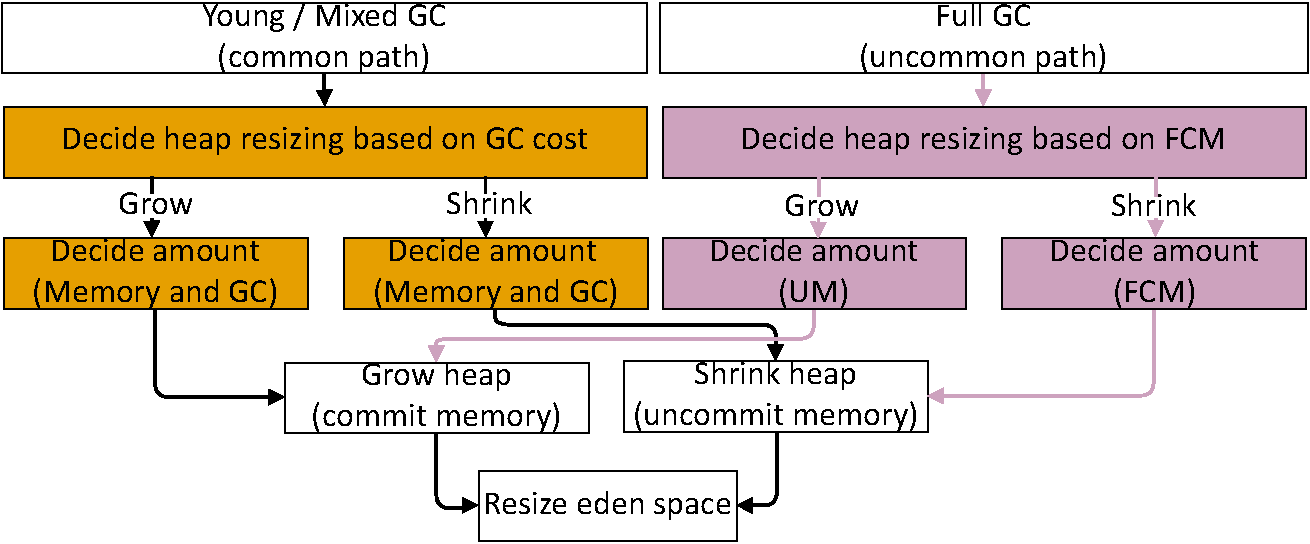
\includegraphics[width=0.56\linewidth]{flexheap/fig/design/g1_policy.pdf}}
	\subfloat[\flexheapName{}]{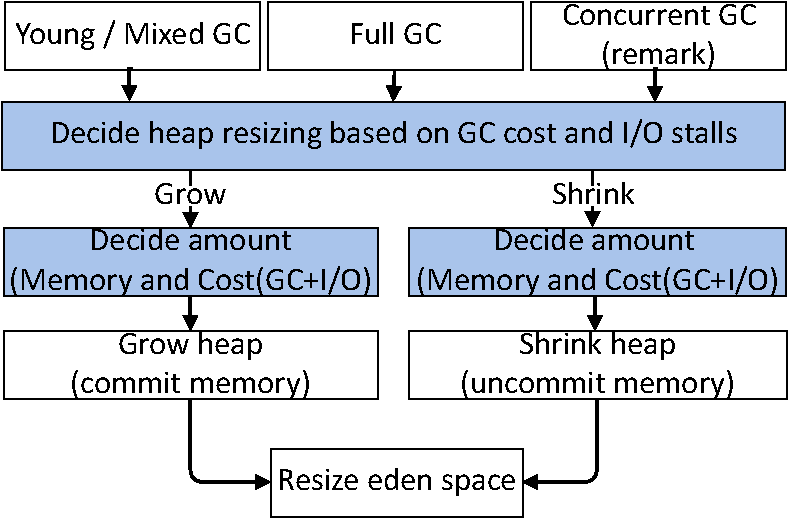
\includegraphics[width=0.355\linewidth]{flexheap/fig/design/fh_policy.pdf}}
	\caption{Overview of (a) G1 and (b) \flexheapName{} heap resizing mechanisms (acronyms:
		%
		\textbf{UM}=\textbf{U}ncommitted \textbf{M}emory,
		%
		\textbf{FCM}=\textbf{F}ree \textbf{C}ommitted \textbf{M}emory
	}
	\label{fig:arch}
\end{figure}

Figure~\ref{fig:arch}(b) illustrates the heap resizing mechanism of \flexheapName{} in G1.
We use a unified resizing mechanism regardless of the \flexheapGC{} type.
At each decision point, \flexheapName{}
%
(i) estimates the cost of GC (Section~\S~\ref{sec:gc_cost}) and I/O stalls (Section~\S~\ref{sec:io_cost}),
%
(ii) it uses the combined GC and I/O cost to grow or shrink the heap (Section~\S~\ref{sec:policy}), and
%
(iii) estimates the amount of memory to reassign (Section~\S~\ref{sec:resizing_step}).
%
Next, we discuss each mechanism of \flexheapName{} in more detail.

\subsection{Estimating Impact of \flexheapGC{}}
\label{sec:gc_cost}

\flexheapGC{} activity is the dominant overhead for heap operations.
We estimate the \flexheapGC{} CPU cycles spent in the current interval, defined as the time from the end of $\mathrm{STW}_{i-1}$ to the end of $\mathrm{STW}_{i}$.
Within this interval, we account for all \flexheapGC{} work: the concurrent \flexheapGC{} executed between pauses and the subsequent STW collection (young, mixed, or full GCs).
This concurrent activity includes the concurrent marking \flexheapGC{} cycle, and the work of concurrent refinement threads that update per-region remembered sets.
As the concurrent \flexheapGC{} overlaps with mutators, wall-clock time overestimates actual CPU usage.
Thus, we measure \flexheapGC{} cost in CPU time, following prior work~\cite{zgc:heap_resize}.
The total \flexheapGC{} CPU time of the current interval is the sum of CPU time spent in the subsequent STW \flexheapGC{}s and in concurrent \flexheapGC{}s:

\begin{align}
	\label{eq:gc_cost}
	\mathit{C}_\mathit{gc} = \mathit{C}_\mathit{stw} + \mathit{C}_\mathit{conc}
\end{align}

\paragraph{\textbf{STW GC CPU time}}
During an STW GC, all mutator threads are suspended, so the system loses the computation they could have performed during the pause time ($T_\mathit{stw}$).
The lost computation depends on the minimum of the available CPU cores ($N$) and the number of mutator threads ($M$).
The challenge is knowing $M$ at the pause boundary, as the mutator threads start and terminate over time, and some may already be waiting on locks.
\flexheapName{} therefore uses a practical upper bound: it maintains an atomic count of active Java mutator threads (excluding VM/GC/internal threads), incremented on thread start and decremented on termination, and reads this count at each STW boundary.
This may overestimate lost work because some counted threads could be non-runnable, but filtering them out would require a pre-safepoint runnability snapshot and per-transition instrumentation, adding prohibitive overhead.
Thus, we compute the STW cost as:

\begin{align}
	\label{eq:gc_stw}
	\mathit{C}_\mathit{stw} = T_\mathit{stw} \cdot \min(N, M)
\end{align}

\paragraph{\textbf{Concurrent GC CPU time}}
During concurrent \flexheapGC{}, both mutator and \flexheapGC{} threads execute in parallel and contend for CPU resources.
We estimate the portion of $G$ concurrent \flexheapGC{} threads that displace work from $M$ mutator threads, resulting in lost mutator progress.
$G$ includes both concurrent marking threads and refinement threads.
For this purpose, \flexheapName{} compares the total number of active threads ($M + G$) to the number of available cores $N$ for the specific interval.
When $M + G \leq N$, there are idle cores, and concurrent \flexheapGC{} can proceed without cost.
When $M + G > N$, some \flexheapGC{} threads preempt mutators, and only the excess CPU time beyond idle capacity contribute to overhead.
The concurrent cost is therefore:

\begin{align}
	\label{eq:conc_gc}
	\mathit{C}_\mathit{conc} =
	\begin{cases}
		\displaystyle \sum_{g \in G} T_{\mathrm{CPU}}(g) - \max\bigl(0,\,(N - M)\cdot T_\mathit{mut}\bigr), & M + G > N    \\
		0,                                                                                                  & M + G \leq N
	\end{cases}
\end{align}

Here, $T_\mathit{mut}$ is the time between the end of one STW phase and the start of the next, representing the interval during which mutator and concurrent GC threads overlap.
For example, on an 8-core system, suppose that during a given interval there are $M = 6$ mutators and $G = 4$ concurrent GC threads.
With $N = 8$, only $N - M = 2$ cores are available for concurrent GC, so $G - (N - M) = 2$ concurrent GC threads have no idle cores to run on; their CPU cycles in that interval are counted as overhead.
In addition to competing for cores, concurrent GC threads can also interfere with mutators through contention for other resources, such as cache and memory.
Precisely attributing that interference would require fine-grained hardware profiling which adds non-negligible overhead and complexity.

\subsection{Estimating Impact of I/O Stalls}
\label{sec:io_cost}
The memory available to the I/O cache directly determines how much time mutator threads spend stalled on I/O.
A larger I/O cache allows more frequently accessed data to be served from DRAM, reducing page faults that cause storage access and keeping mutators from getting context switched.
However, this benefit depends on the access locality: workloads with little or no reuse derive limited advantage from additional cache space.
Conversely, when the I/O cache is small or under pressure, a larger fraction of reads and writes must be served from the storage device, causing mutator threads to block in the kernel I/O path until the data are fetched into memory.
These stalls translate directly into CPU time that could otherwise be used for application processing, reducing performance.
To capture this effect, \flexheapName{} estimates the CPU time lost due to I/O stalls, using it as a measure of the performance cost of limited I/O cache space to guide resizing decisions.

\begin{algorithm}
	\caption{eBPF Handler for \texttt{sched\_switch}.}
	\begin{algorithmic}[1]
		\Procedure{on\_sched\_switch}{prev\_tid, next\_tid, prev\_state}
		\State ts $\gets$ current\_time()

		\If {prev\_tid $\in$ mutators \textbf{and} prev\_state = D}
		\State iostart[prev\_tid] $\gets$ ts
		\EndIf

		\If {next\_tid $\in$ mutators \textbf{and} next\_tid $\in$ iostart}
		\State dt $\gets$ ts $-$ iostart[next\_tid]
		\If{next\_tid $\in$ iowait}
		\State iowait[next\_tid] $\gets$ iowait[next\_tid] $+$ dt
		\Else
		\State iowait[next\_tid] $\gets$ dt
		\EndIf
		\State \textbf{delete} iostart[next\_tid]
		\EndIf
		\EndProcedure
	\end{algorithmic}
	\label{alg:ebpf}
\end{algorithm}

To quantify this loss, we measure the time mutator threads spend in the uninterruptible (D) state~\cite{kernel:sleeping}, during which they are blocked on I/O and cannot make progress.
Even when other threads continue to use the CPUs, these stalled mutators still represent lost opportunities for mutator progress.
$C_\mathit{io}$ therefore captures mutator progress lost while threads are blocked on I/O.
This differs from $C_\mathit{gc}$, which estimates the loss caused by \flexheapGC{} displacing runnable mutators from the CPU.
Measuring $C_\mathit{io}$ only as idle-core-equivalent stall time would therefore underestimate the impact of I/O-bound phases, particularly in services where blocked mutators contribute to queue buildup and tail latency.

% \flexheapName{} requires a per-mutator-thread approximation of I/O stall time, which
% standard kernel interfaces do not directly expose. The \texttt{iowait} metric in
% \texttt{/proc/stat} is insufficient for this purpose because it is a CPU-level
% aggregate metric: it indicates that a CPU is idle while at least one task is
% waiting for I/O~\cite{linux:iowait}, rather than the stall time of a specific
% thread. Thus, a mutator may be blocked on a lock while an unrelated task on the
% same CPU waits for I/O, making \texttt{iowait} an incorrect proxy for the
% mutator's I/O stall time. More fundamentally,

Existing standard kernel interfaces do not directly expose the time per mutator thread lost to I/O stalls.
The \texttt{iowait} metric in \texttt{/proc/stat} is a CPU-level aggregate metric.
It reports that a CPU is idle while at least one task is waiting for I/O~\cite{linux:iowait}, rather than how much time a particular thread is stalled on I/O.
For example, a mutator thread may be blocked on a lock while an unrelated thread on the same CPU waits for I/O, so treating the recorded \texttt{iowait} as the mutator's I/O stall time would be incorrect.
More fundamentally, kernel interfaces do not directly expose per-thread I/O stall measurements, because scheduler semantics decouple I/O completion from rescheduling.
For example, a thread's I/O may complete before the scheduler places the thread back on a CPU, making it unclear whether the intervening delay should be counted as I/O stall time.

\flexheapName{} implements an eBPF~\cite{ebpf} program attached to the \texttt{sched\_switch} tracepoint to obtain an approximation of the per mutator thread I/O stall time, as shown in Algorithm~\ref{alg:ebpf}.
The eBPF program maintains two maps: \texttt{iostart}, which stores the timestamp at which a mutator thread enters the D state, and \texttt{iowait}, which accumulates the total time that the thread has spent blocked on I/O.
On each context switch, if a tracked mutator thread is scheduled out in the D state, we record the current timestamp in \texttt{iostart}; when it is scheduled back in, we compute the elapsed time since that timestamp and add it to \texttt{iowait}.
We use the accumulated value in \texttt{iowait} as the mutator CPU time lost to I/O stalls.

To ensure the estimate respects hardware limits, the computed I/O-induced CPU time loss must not exceed the machine’s compute capacity over the measurement interval.
When the number of mutator threads exceeds the available CPU cores and all are simultaneously stalled on I/O, the total lost CPU time cannot be greater than the interval duration multiplied by the number of cores.
We therefore cap the measured stall time to the product of the interval duration and the number of CPU cores, as shown in Eq.~\ref{eq:io}:

\begin{equation}
	\label{eq:io}
	\mathit{C}_\mathit{io} = \min \bigl(\displaystyle \sum_{m \in M} T_{\mathrm{io}}(m), T_\mathit{mut} \cdot N \bigr)
\end{equation}

\subsection{Deciding to Grow or Shrink the Heap}
\label{sec:policy}

% FlexHeap uses a feedback-driven, model-free controller because the relationship
% between heap size, GC overhead, and I/O-cache benefit is highly sensitive to
% the workload phase and system environment. In particular, shrinking the heap
% does not imply a fixed or proportional reduction in I/O cost: the resulting
% benefit depends on the application's access pattern, working-set size, storage
% characteristics, and whether the memory released from the heap is actually
% available to and beneficial for the page cache. While a model-based design
% could potentially adapt faster when its assumptions hold, FlexHeap instead
% prioritizes robustness across workloads and storage environments by reacting to
% observed changes in GC and I/O cost.

After each \flexheapGC{} cycle, \flexheapName{} determines whether to grow the heap (\texttt{growHeap}) or shrink the heap (\texttt{shrinkHeap}) to release memory for the I/O cache.
For the decision-making process, \flexheapName{} compares, across intervals, the sum of CPU time consumed by \flexheapGC{} and I/O stalls, which together capture lost mutator progress.
To reduce short-term noise, \flexheapName{} averages the sum of $C_\mathit{gc}$ and $C_\mathit{io}$ over the last ten intervals, following G1's use of a ten-interval moving average.
An alternative approach would be to balance these two costs, aiming for equal contribution from both.
However, this does not necessarily minimize total overhead.
Equalizing the two costs may still yield suboptimal performance.
For example, in scan-heavy workloads with low I/O cache hit rates, prioritizing I/O cost could enlarge the I/O cache without improving throughput, while simultaneously inflating \flexheapGC{} overhead.
This counterproductive behavior shows that balancing costs is insufficient—\flexheapName{} instead seeks to reduce their combined sum.

% Summing these two costs has two benefits. First, it directly reduces total
% overhead, whereas balancing \flexheapGC{} and I/O stall costs does not necessarily
% reduce end-to-end performance loss. For example, in scan-heavy workloads with
% low I/O-cache hit rates, prioritizing I/O cost could enlarge the I/O cache
% without improving throughput, while simultaneously increasing \flexheapGC{} overhead.
% Second, it avoids introducing explicit weights for each cost. A weighted
% formulation would require tuning the relative importance of heap-related and
% cache-related effects, which may vary across workloads and execution phases.

If a \texttt{shrinkHeap} (or \texttt{growHeap}) action reduces the total cost ($C_\mathit{tot} = C_\mathit{gc} + C_\mathit{io}$), \flexheapName{} continues applying the same action.
However, whenever \flexheapName{} applies a resize action, it must account for the delay before the effects of the previous resize are reflected in heap usage or I/O cache growth.
Without waiting for the repurposed memory to be absorbed by the heap or the I/O cache, \flexheapName{} could issue premature actions, resulting in unnecessary or even harmful resizing.
This is particularly important when memory released from the heap does not improve the I/O cache, for example because the application uses direct I/O, or because, in a multitenant container, the freed memory is consumed by sibling processes instead.

\begin{figure}[t]
	\centering

	\begin{minipage}{\linewidth}
		\centering
		\resizebox{0.65\linewidth}{!}{%
			\begin{tabular}{ccc}
				\toprule
				\textbf{Predicate}                                                              &
				\textbf{Predicate Definition}                                                   &
				\textbf{Complementary Predicate}                                                  \\
				\midrule
				\texttt{costDown}                                                               &
				$C_\mathrm{tot}[t] \leq C_\mathrm{tot}[t-1]$                                    &
				\texttt{costUp}                                                                   \\
				\texttt{growSlack}                                                              &
				$S_\mathrm{used} < S_\mathrm{used\_before\_grow} + S_\mathrm{grow}$             &
				\texttt{growUsed}                                                                 \\
				\texttt{ioSlack}                                                                &
				$S_\mathrm{io} < S_\mathrm{io\_before\_shrink} + S_\mathrm{shrink}$             &
				\texttt{ioFull}                                                                   \\
				\texttt{gcBias}                                                                 &
				$\Delta^\mathrm{rel} C_\mathrm{gc}[t] \ge \Delta^\mathrm{rel} C_\mathrm{io}[t]$ &
				\texttt{ioBias}                                                                   \\
				\bottomrule
			\end{tabular}%
		}
	\end{minipage}

	\vspace{0.8em}

	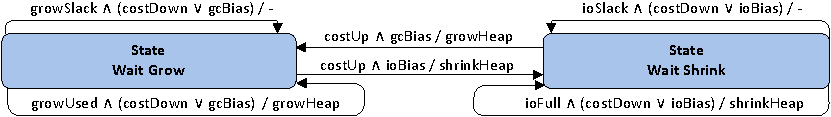
\includegraphics[width=\linewidth]{flexheap/fig/design/fh_logic.pdf}
	\caption{Finite-state machine of the FlexHeap resizing controller.
Each transition label has the form \textit{condition} / \textit{action}.
The table defines the predicates used in transition guards, their formal definitions, and the complementary predicate names.
For example, \texttt{growUsed} is the complement of \texttt{growSlack} and denotes the case where the heap has exhausted the space added by the previous grow step.
In the table, for the definition of predicates, $S$ denotes a size-related quantity.}
	\label{fig:fsm}
\end{figure}

To handle delayed effects, \flexheapName{} employs \emph{wait states}, which defer further resizing until the impact of the previous action becomes observable, as shown in Figure~\ref{fig:fsm}.
After a \texttt{growHeap} action, \flexheapName{} enters in the state \emph{Wait Grow}.
If $C_\mathit{tot}$ decreases and the space added by the previous grow step has not yet been exhausted (\texttt{growSlack}), the controller waits; if that space has been exhausted (\texttt{growUsed}), it issues another \texttt{growHeap} action.
Symmetrically, after a \texttt{shrinkHeap} action, \flexheapName{} enters in the state \emph{Wait Shrink}.
If $C_\mathit{tot}$ decreases and the memory released by the previous shrink step has not yet been fully consumed by the I/O cache (\texttt{ioSlack}), the controller waits; otherwise, it issues another \texttt{shrinkHeap} action.

Conversely, if $C_\mathit{tot}$ increases, \flexheapName{} determines the next direction by comparing the relative change of the two cost components, denoted by $\Delta^{\mathrm{rel}} C_x[t] = (C_x[t] - C_x[t-1]) / C_x[t-1]$.
If the relative change in $C_\mathrm{gc}$ is greater than or equal to that in $C_\mathrm{io}$ (\texttt{gcBias}), the controller infers that GC was affected more adversely by the last resizing step and issues \texttt{growHeap}; otherwise, it issues \texttt{shrinkHeap}.
We use relative rather than absolute changes because $C_\mathrm{gc}$ and $C_\mathrm{io}$ may differ by orders of magnitude and their dominance may shift across workloads and phases.
Comparing absolute values would bias the controller toward whichever component is currently larger, even when the other is more sensitive to heap resizing.
By normalizing each cost to its previous value, \flexheapName{} makes scale-invariant decisions based on which component changed more sharply in response to the last action.

A simpler alternative would be to immediately undo the previous resizing action whenever $C_\mathit{tot}$ increases.
We do not adopt this policy because such an immediate reversal may be premature and can induce oscillation.
$C_\mathit{gc}$ and $C_\mathit{io}$ respond differently to memory reassignment: additional heap memory generally reduces GC pressure, whereas releasing memory to the I/O cache does not always reduce I/O cost, depending on the workload’s working-set size and access pattern.

\paragraph{\textbf{Proactive GC triggering during mutator I/O stalls}}
Mutator threads can become blocked on I/O for an extended period, significantly delaying the next GC cycle.
When this happens, heap resizing decisions are also delayed, leading to feedback lag.
To maintain responsiveness in these cases, \flexheapName{} triggers a GC proactively when mutator threads stall as follows.

A lightweight VM thread runs periodically every second (similar to VG1) and monitors two runtime metrics: allocation rate and mutator I/O stall time.
\flexheapName{} samples the total bytes allocated by mutator threads every second.
It maintains a sliding window of recent allocation measurements and computes a moving average over the last five intervals.
If the current allocation rate drops by half, \flexheapName{} marks the interval as a low-activity period.
To avoid reacting to transient changes, it tracks how many of the last few intervals have shown low activity.
Only if multiple consecutive samples indicate reduced allocation rate, does it consider the system to be stalled.
For this period, \flexheapName{} also monitors I/O stall cycles.
If high stall time coincides with low allocation activity, \flexheapName{} concludes that threads are waiting on I/O rather than idle, and triggers a GC.
To avoid disrupting normal GC scheduling, \flexheapName{} inserts the GC request through standard internal JVM hooks, and ensures that no GC is already in progress.

\subsection{Estimating the Resizing Step}
\label{sec:resizing_step}

The goal of the growing and shrinking steps is to respond quickly to changes in application behavior and to respect G1’s pause time goals.
For responsiveness, \flexheapName{} scales each resize step by the recent change in the combined cost.
For pause protection, \flexheapName{} relies on G1’s eden sizing model and leaves it unchanged.
This model is not part of our resizing mechanism.
After each young or mixed \flexheapGC{}s, G1 measures the pause overhead.
It uses this metric to predict the next young-GC pause and then chooses the largest size for eden space that meets the user pause target within available free memory.
We use this model only to bound shrinking: the shrink step returns memory only from free regions beyond the computed target size of eden space.
Similar to G1’s resizing mechanism, we do not use the pause-time model for the growth step.
Growing only adds free regions, and G1’s eden sizing model still selects exactly as many eden regions as needed to meet the pause target.
Growth therefore follows G1’s bounded expansion mechanism, scaled by our total cost metric, while remaining aligned to region size and limited by uncommitted headroom.

\begin{figure}[h]
	\centering
	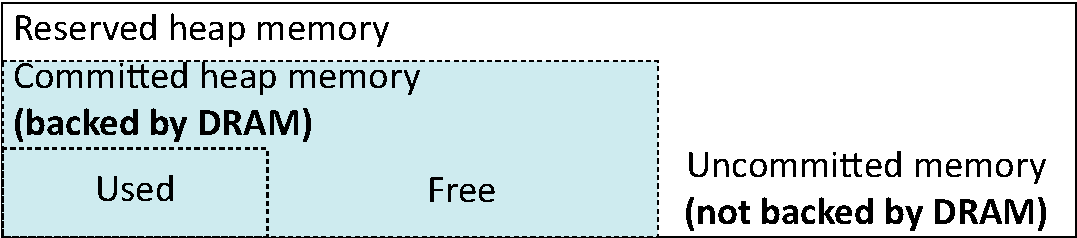
\includegraphics[width=0.5\linewidth]{flexheap/fig/design/jvm_mem.pdf}
	\caption{Committed and uncommitted heap memory.}
	\label{fig:jvm_mem}
\end{figure}

\begin{algorithm}[h]
	\caption{Growing step}
	\label{alg:growth_step}
	\begin{algorithmic}[1]
		\Procedure{grow\_amount}{$\Delta C_{\text{tot}}$}
		\State \texttt{reserved} \(\gets\) \texttt{max\_capacity}()
		\State \texttt{committed} \(\gets\) \texttt{capacity}()
		\State \texttt{uncommitted} \(\gets\) \texttt{reserved} \(-\) \texttt{committed}
		\State \texttt{expand\_via\_pct} \(\gets\) \texttt{G1ExpandByPercentOfAvailable} \(\times\) \texttt{uncommitted}
		\State \texttt{min\_expand} \(\gets \min(\texttt{RegionSize},\ \texttt{uncommitted})\)
		\State \texttt{resize\_bytes} \(\gets \min(\texttt{expand\_via\_pct},\ \texttt{committed})\) \label{line:resize}
		\State \texttt{scale\_factor} \(\gets\) \texttt{scale\_total\_cost\_delta}(\(\Delta C_{\text{tot}}\), \texttt{MinScaleFactor}, \texttt{MaxScaleFactor}) \label{line:scale}
		\State \texttt{resize\_bytes} \(\gets \texttt{resize\_bytes} \times \texttt{scale\_factor} \)
		\State \textbf{return} \(\max\!\big(\min(\texttt{resize\_bytes}, \texttt{uncommitted}), \texttt{min\_expand}\big)\)
		\EndProcedure
	\end{algorithmic}
\end{algorithm}

\paragraph{\textbf{Growing step}}
As shown in Figure~\ref{fig:jvm_mem}, the heap has committed memory (backed) and uncommitted memory (reserved up to maximum heap size).
A grow step, calculated by Algorithm~\ref{alg:growth_step}, cannot exceed the uncommitted headroom.
\flexheapName{} forms a base budget as the smaller of (i) a fixed percentage of the uncommitted headroom (the same percentage used by native G1) and (ii) the current committed size (Line~\ref{line:resize}).
This avoids oversized jumps that would reduce \flexheapGC{} frequency and risk longer pauses.
\flexheapName{} then scales the normalized cost change $\Delta C_{\text{tot}}$ using a step scale with a logistic (S-shaped) function (Line~\ref{line:scale}).
$\Delta C_{\text{tot}}$ is the change between intervals: larger increases yield larger steps, small changes yield conservative steps.
We adopt the same logistic form used by G1’s resizing mechanism, keeping tuning behavior consistent.
Finally, \flexheapName{} returns the grow bytes constrained to the admissible range.
The resize amount does not exceed the available uncommitted headroom and is not less than the minimum expansion.

\paragraph{\textbf{Shrinking step}}
Algorithm~\ref{alg:shrink_step} describes the computation for the shrink step.
We first use G1’s pause-time model to compute the number of regions needed to meet the eden target length (Line~\ref{line:eden}).
Then, we subtract it from the current number of free regions to obtain the shrinkable budget (Line~\ref{line:free}).
This respects G1’s pause time goal by not reducing eden below the target G1 selects.
We then ,similar to growing step, we scales the normalized cost change $\Delta C_{\text{tot}}$ using a step scale with a logistic (S-shaped) function (Line~\ref{line:scale2}).
Finally, we convert the shrinkable regions to bytes, and multiply by the scale factor to obtain the shrink amount.

\begin{algorithm}[h]
	\caption{Shrinking step}
	\label{alg:shrink_step}
	\begin{algorithmic}[1]
		\Procedure{shrink\_amount}{$\Delta C_{\text{tot}}$}
		\State \texttt{regions\_to\_shrink} \(\gets\) \texttt{num\_free\_regions}()
		\State \texttt{regions\_for\_eden\_space} \(\gets\) \texttt{eden\_target\_length}() \label{line:eden}
		\State \texttt{regions\_to\_shrink} \(\mathrel{-}= \texttt{regions\_for\_eden\_space}\) \label{line:free}
		\State \texttt{scale\_factor} \(\gets\) \texttt{scale\_total\_cost\_delta}(\(\Delta C_{\text{tot}}\), \texttt{MinScaleFactor}, \texttt{MaxScaleFactor}) \label{line:scale2}
		\State \texttt{resize\_bytes} \(\gets \texttt{regions\_to\_shrink} \cdot \texttt{RegionSize} \cdot \texttt{scale\_factor}\)
		\State \textbf{return} \(\texttt{resize\_bytes}\)
		\EndProcedure
	\end{algorithmic}
\end{algorithm}

% An interesting direction for future work is to augment the resizing step with a
% different model that estimates how much memory should be reallocated to the
% heap or to the I/O cache by capturing how useful additional memory is in each
% case. Such a model could also incorporate weights that reflect the relative
% importance of GC cost and I/O stalls.
